
Das E-R Modell wird oft als Werkzeug in der konzeptuellen Designphase eingesetzt. Jedes E-R Modell lässt sich in ein relationales Schema übersetzen.
\subsection{Elemente}
\subsubsection*{Entitäten und Entitätsmengen}
\begin{mybox}[title=Entität]
Eine \Gls{Entität} stellt ein real oder virtuell existierendes Element in der Welt dar, welches eindeutig von anderen Elementen unterschieden werden kann.
\end{mybox}
Eine Entitätsmenge ist eine Menge von Entitäten mit gleichen Eigenschaften. Wir bezeichnen die Gesamtheit aller Entitäten einer Entitätsmenge als ihre \Gls{Extension}.
\begin{figure}[H]
    \centering
    \begin{subfigure}{0.3\textwidth}
    
\includegraphics[width=\textwidth]{images/entität.png.png}
    \caption{Normale Entität.}
    \label{fig:entität}
    \end{subfigure}
    \begin{subfigure}{0.3\textwidth}
    
\includegraphics[width=\textwidth]{images/schwacheentität.png.png}
    \caption{Schwache Entität.}
    \label{fig:schwentität}
    \end{subfigure}
    \caption{Darstellungsweisen der verschiedenen Typen von Entitäten in E-R-Modellen.}
    \label{fig:entitäten}
\end{figure}
\Gls{Schwache Entitätsmenge}
\Gls{Identifizierende Entitätsmenge}
\Gls{Starke Entitätsmenge}
\Gls{Diskriminator}
\subsubsection*{Attribute}
Eine \Gls{Entität} wird beschrieben durch eine Menge von Attributen. \Glspl{Attribut} sind beschreibende Merkmale, die auf alle Entitäten in einer Entitätsmenge zutreffen.
\begin{mybox}[title=Schlüsselattribut]
Schlüsselattribute sind Attribute, die eindeutig sind in dem Sinne, dass alle Entitäten in einer Entitätsmenge verschiedene Werte für dieses Attribut annehmen.
\end{mybox}
\begin{figure}[H]
    \centering
    \begin{subfigure}{0.3\textwidth}
    
\includegraphics[width=\textwidth]{images/einwertattr.png}
    \caption{Einwertiges Attribut.}
    \label{fig:attribut}
    \end{subfigure}
    \begin{subfigure}{0.3\textwidth}
    
\includegraphics[width=\textwidth]{images/mehrwertattr.png}
    \caption{Mehrwertiges Attribut.}
    \label{fig:mehrattribut}
    \end{subfigure}
    \begin{subfigure}{0.3\textwidth}
    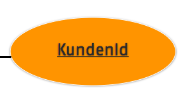
\includegraphics[width=\textwidth]{images/schlattr.png}
    \caption{Schlüsselattribut.}
    \label{fig:schlattribut}
    \end{subfigure}
    \begin{subfigure}{0.3\textwidth}
    
\includegraphics[width=\textwidth]{images/abglattr.png}
    \caption{Abgeleitetes Attribut.}
    \label{fig:abgelattr}
    \end{subfigure}
    \begin{subfigure}{0.5\textwidth}
    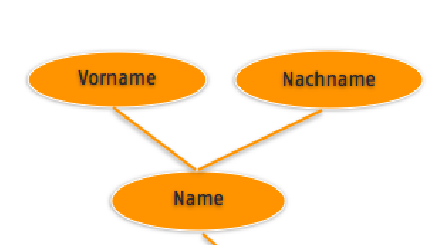
\includegraphics[width=\textwidth]{images/zsmgesattr.png}
    \caption{Zusammengesetztes Attribut.}
    \label{fig:zsmgesattr}
    \end{subfigure}
    \caption{Darstellungsweisen der verschiedenen Typen von Attributen in E-R-Modellen.}
    \label{fig:attribute}
\end{figure} \noindent
Für jedes Attribut $A$ einer Entitätsmenge $E$ müssen die gültigen Werte spezifiziert werden. Dies geschieht durch Angabe eines Wertebereiches oder \Gls{Domäne}. \\
$D_A$ ist dabei die Domäne des Attributes $A$. Ein Attribut ist formal eine Funktion, die jeder Entität einen Wert zuweist: 
\begin{equation*}
    f_A : E \rightarrow D_A
\end{equation*}
Jede Entität hat konkrete Werte für ihre verschiedenen Attribute!
\subsection{Beziehungen und Beziehungsmengen}
Eine Beziehung verbindet mehrere Entitäten. Eine \Gls{Beziehungsmenge} ist eine Menge von Beziehungen des gleichen Typs (d.h. zwischen den gleichen Typen von Entitäten). \\ Formal gesehen entspricht eine Beziehungsmenge $R$ zwischen Entitätsmengen $E_1, ..., E_n$ mit $n \geq 2$ einer Teilmenge des kartesischen Produktes $E_1 \times E_2 \times ... \times E_n$, d.h.
\begin{equation*}
    R \subseteq E_1 \times E_2 \times ... \times E_n
\end{equation*}
\begin{mybox}[title=Instanz einer Beziehungsmenge]
Eine \Gls{InstB} repräsentiert eine konkrete Verbindung zwischen zwei Entitäten.
\end{mybox}

\begin{figure}[H]
    \centering
    \begin{subfigure}{0.3\textwidth}
    %\includegraphics[width=\textwidth]{images/}
    \caption{Vollständige Beziehung.}
    \label{fig:vollstB}
    \end{subfigure}
    \begin{subfigure}{0.3\textwidth}
    %\includegraphics[width=\textwidth]{images/}
    \caption{Rekursive Beziehungsmenge.}
    \label{fig:rekB}
    \end{subfigure}
    \begin{subfigure}{0.3\textwidth}
    %\includegraphics[width=\textwidth]{images/}
    \caption{Binäre Beziehung.}
    \label{fig:binB}
    \end{subfigure}
    \begin{subfigure}{0.3\textwidth}
    %\includegraphics[width=\textwidth]{images/}
    \caption{Höhergradige Beziehung.}
    \label{fig:höhB}
    \end{subfigure}
    \begin{subfigure}{0.3\textwidth}
    %\includegraphics[width=\textwidth]{images/}
    \caption{Identifizierende Beziehung.}
    \label{fig:identB}
    \end{subfigure}
    \caption{Darstellungsweisen der verschiedenen Typen von Beziehungen in E-R-Modellen.}
    \label{fig:beziehungen}
\end{figure} \noindent
\subsubsection*{Beschränkungen der Beteiligung}
\begin{mybox}[title=Kardinalitäten in Intervallnotation]
\Glspl{Kardinalitäten} werden verwendet, um die Beteiligung zu beschränken, insbesondere um die Anzahl der Relationen einzuschränken, an der eine Entität teilnehmen kann. Wir verwenden dafür
eine \Gls{Intervallnotation} und markieren mit dem entsprechenden Intervall die Kante zwischen Be-
ziehungsmenge $R$ und beteiligter Entitätsmenge $E_i$. Wenn die Beteiligung von Entität $E_i$ an der Beziehungsmenge $R$ mit dem Intervall [min..max] eingeschränkt ist, dann bedeutet das, dass, jede Entität $e \in E$ an minimal min und maximal max Beziehungen beteiligten sein kann, oder auch formaler für eine Beziehungsmenge $R$ mit n beteiligten Entitäten $E1, ..., En$:
\begin{equation}
\forall e_i \in E_i : \min \leq \#\{(e_1, e_2, \dots, e_{i-1}, e_{i+1}, \dots, e_n) \mid (e_1, e_2, \dots, e_{i-1}, e_i, e_{i+1}, \dots, e_n) \in R\} \leq \max
\end{equation}
\end{mybox}
\begin{table}[H]
    \centering
    \begin{tabular}{l l p{10cm}}
        many-to-many &  m:n & \\
        one-to-many & 1:n & Eine Beziehungsmenge R ist one-to-many oder 1:n von E1 nach E2 wenn eine Entität aus E1 mit mehreren Entitäten aus E2 in Beziehung stehen kann, aber eine Entität aus E2 mit höchstens einer Entität aus E1 in Beziehung stehen kann, wobei E1 und E2 an R beteiligte Entitätsmengen sind. \\
        many-to-one & n:1 & Eine Beziehungsmenge R ist many-to-one oder n:1 von E1 nach E2 wenn eine Entität aus E1 mit höchstens einer Entität aus E2 in Beziehung stehen kann aber eine Entität aus E2 mit mehreren Entitäten aus E1 in Beziehung stehen kann, wobei E1 und E2 an R beteiligte Entitätsmengen sind. \\
        one-to-one & 1:1 & Eine Beziehung R ist one-to-one (bzw. 1:1) von E1 nach E2 wenn eine Entität aus E1 mit höchstens einer Entität aus E2 in Beziehung stehen kann und eine Entität aus E2 mit höchstens einer Entität aus E1 in Beziehung stehen kann. Hierbei sind E1 und E2 an R beteiligte Entitätsmengen.
    \end{tabular}
    \caption{Arten von Kardinalitäten.}
    \label{tab:kardinalitäten}
\end{table} \noindent
\subsubsection*{Vererbung}
\Gls{Generalisierung}
\Gls{Spezialisierung}
\Gls{einfache Vererbung}
\Gls{mehrfache Vererbung}
\Gls{disjunkte Vererbung}
%\Gls{überlappende Spezialisierung }
\Gls{überlappende Generalisierung}
\Gls{Vollständige Spezialisierung}

\begin{figure}[H]
    \centering
    \begin{subfigure}{0.3\textwidth}
   % \includegraphics[width=\textwidth]{images/}
    \caption{Normale Vererbungshierarchie.}
    \label{fig:isa}
    \end{subfigure}
    \begin{subfigure}{0.3\textwidth}
   % \includegraphics[width=\textwidth]{images/}
    \caption{Disjunkte Vererbungshierarchie.}
    \label{fig:disa}
    \end{subfigure}
    \label{fig:isas}
\end{figure} \noindent


\subsection{Interpretation von ER Modellen}
\subsubsection*{Kardinalitäten auslesen}
\begin{figure}[H]
    \centering
    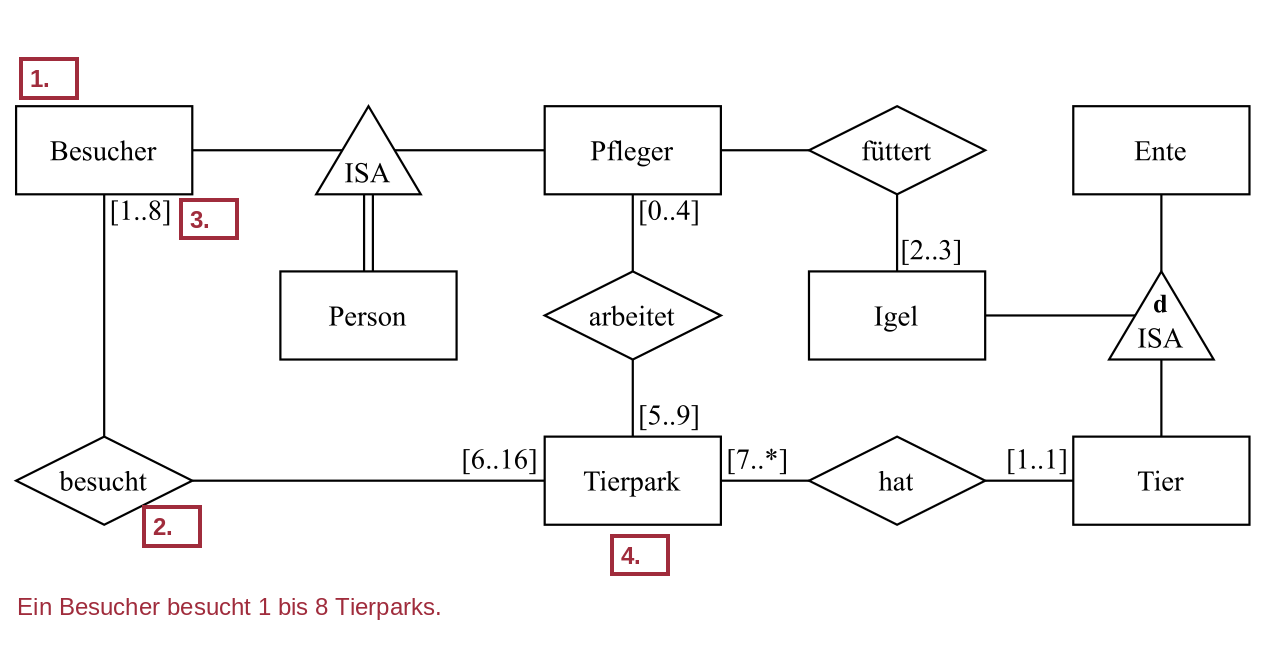
\includegraphics[width=15cm]{images/Zoo1.png}
    \caption{Auslesen von einfachen Kardinalitäten aus einem E-R-Modell.}
    \label{fig:zooKardEinf}
\end{figure}
\subsubsection*{Überlappungen berechnen}
\begin{figure}[H]
    \centering
     \begin{subfigure}{0.7\textwidth}
       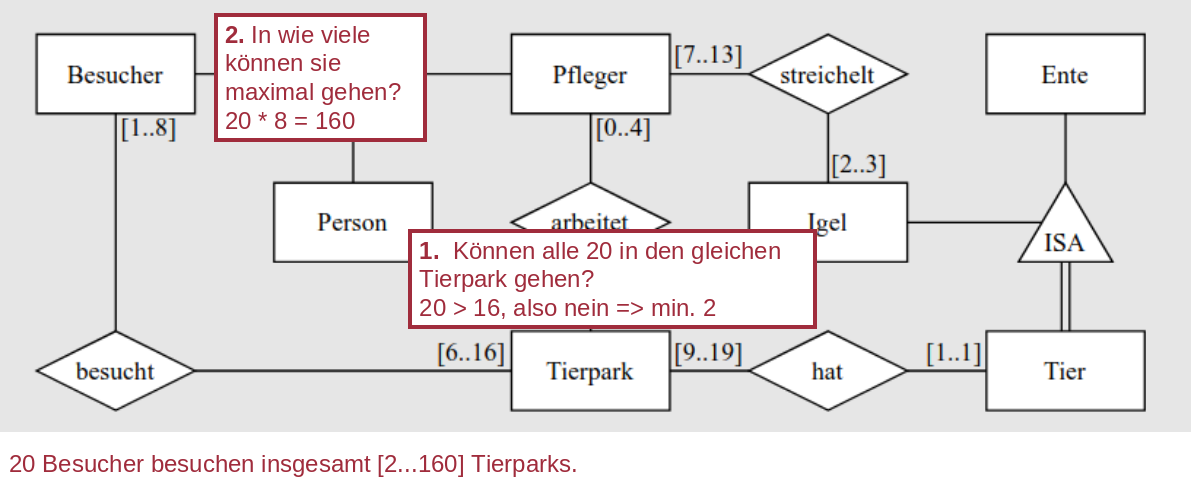
\includegraphics[width=\textwidth]{images/Z002.png}
       \caption{}
    \end{subfigure}
    \begin{subfigure}{0.7\textwidth}
    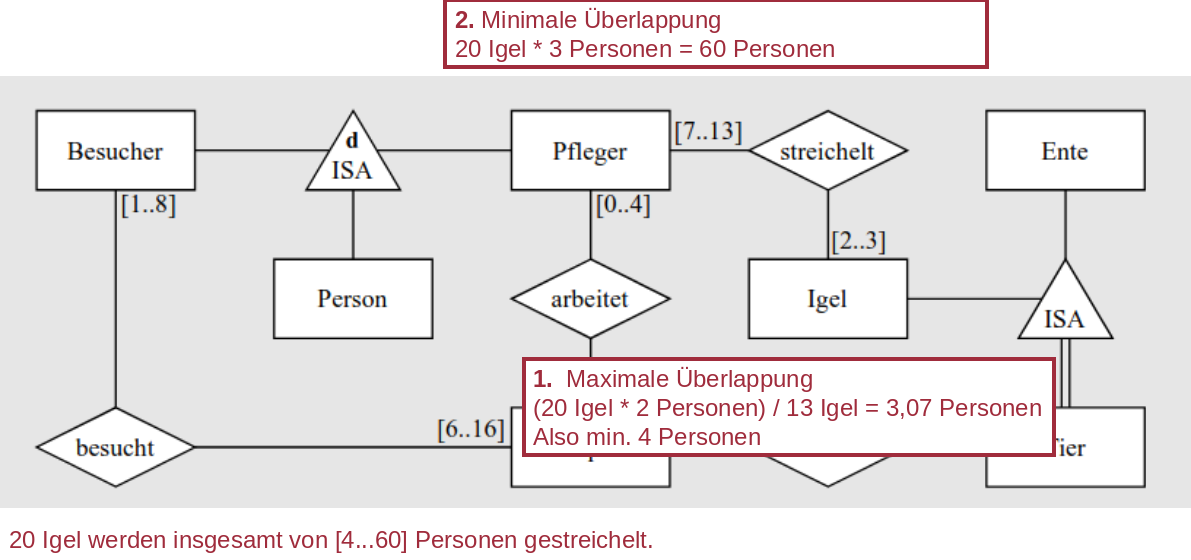
\includegraphics[width=\textwidth]{images/zoo3.png}
    \caption{}
    \end{subfigure}
    \caption{Auslesen von zusammengesetzten Kardinalitäten aus einem E-R-Modell.}
    \label{fig:zooKardZus}
\end{figure}
